\documentclass[8pt]{beamer}
\setbeamerfont{institute}{size=\small}

\newif\ifplacelogo % create a new conditional
\placelogotrue % set it to true

\usetheme{Warsaw}
\usecolortheme{rose}
\usepackage{multicol}
\usepackage{epstopdf}
\usepackage{textcomp}
\usepackage{adjustbox}
\usepackage[italic]{hepnames}
\usepackage{bbding} % for special charachters e.g. for itemize (ftp://ftp.dante.de/tex-archive/fonts/bbding/bbding.pdf)
\usepackage{xcolor}
\usepackage{pdfpages}

% remove navigation buttons
% \beamertemplatenavigationsymbolsempty

% TikZ includes!!!
\usepackage{tikz}
\usepackage[compat=1.1.0]{tikz-feynman}
\usetikzlibrary{backgrounds}
\tikzstyle{every picture}+=[remember picture]
\makeatletter
\def\grd@save@target#1{%
  \def\grd@target{#1}}
\def\grd@save@start#1{%
  \def\grd@start{#1}}
\tikzset{
  grid with coordinates/.style={
    to path={%
      \pgfextra{%
        \edef\grd@@target{(\tikztotarget)}%
        \tikz@scan@one@point\grd@save@target\grd@@target\relax
        \edef\grd@@start{(\tikztostart)}%
        \tikz@scan@one@point\grd@save@start\grd@@start\relax
        \draw[minor help lines] (\tikztostart) grid (\tikztotarget);
        \draw[major help lines] (\tikztostart) grid (\tikztotarget);
        \grd@start
        \pgfmathsetmacro{\grd@xa}{\the\pgf@x/1cm}
        \pgfmathsetmacro{\grd@ya}{\the\pgf@y/1cm}
        \grd@target
        \pgfmathsetmacro{\grd@xb}{\the\pgf@x/1cm}
        \pgfmathsetmacro{\grd@yb}{\the\pgf@y/1cm}
        \pgfmathsetmacro{\grd@xc}{\grd@xa + \pgfkeysvalueof{/tikz/grid with coordinates/major step}}
        \pgfmathsetmacro{\grd@yc}{\grd@ya + \pgfkeysvalueof{/tikz/grid with coordinates/major step}}
        \foreach \x in {\grd@xa,\grd@xc,...,\grd@xb}
        \node[anchor=north] at (\x,\grd@ya) {\pgfmathprintnumber{\x}};
        \foreach \y in {\grd@ya,\grd@yc,...,\grd@yb}
        \node[anchor=east] at (\grd@xa,\y) {\pgfmathprintnumber{\y}};
      }
    }
  },
  minor help lines/.style={
    help lines,
    step=\pgfkeysvalueof{/tikz/grid with coordinates/minor step}
  },
  major help lines/.style={
    help lines,
    line width=\pgfkeysvalueof{/tikz/grid with coordinates/major line width},
    step=\pgfkeysvalueof{/tikz/grid with coordinates/major step}
  },
  grid with coordinates/.cd,
  minor step/.initial=.2,
  major step/.initial=1,
  major line width/.initial=0.7pt,
}
\makeatother

\newcommand{\myCenterBox}[2][pink] {
   {\centering
    \noindent\colorbox{#1}{
	\textbf{#2}
    }\par
  }
}

\newcommand{\mySmallCenterBox}[2][pink] {
   {\centering
    \noindent\colorbox{#1}{
	\textbf{{\small #2}}
    }\par
  }
}

\newcommand{\myVerySmallCenterBox}[2][pink] {
   {\centering
    \noindent\colorbox{#1}{
	\textbf{{\scriptsize #2}}
    }\par
  }
}

\newcommand{\myBox}[2][pink] {
    \noindent\colorbox{#1}{
	\textbf{#2}
    }\par
}

\newcommand{\mySmallBox}[2][pink] {
    \noindent\colorbox{#1}{
	\textbf{{\small #2}}
    }\par
}

\newcommand{\myVerySmallBox}[2][pink] {
    \noindent\colorbox{#1}{
	\textbf{{\scriptsize #2}}
    }\par
}

% do not use backup slides in page counter
\newcommand{\backupbegin}{
   \newcounter{finalframe}
   \setcounter{finalframe}{\value{framenumber}}
}
\newcommand{\backupend}{
   \setcounter{framenumber}{\value{finalframe}}
}

% custom colors
\definecolor{olive}{rgb}{0.3, 0.4, .1}
\definecolor{fore}{RGB}{249,242,215}
\definecolor{back}{RGB}{51,51,51}
\definecolor{title}{RGB}{255,0,90}
\definecolor{dgreen}{rgb}{0.,0.6,0.}
\definecolor{gold}{rgb}{1.,0.84,0.}
\definecolor{JungleGreen}{cmyk}{0.99,0,0.52,0}
\definecolor{BlueGreen}{cmyk}{0.85,0,0.33,0}
\definecolor{RawSienna}{cmyk}{0,0.72,1,0.45}
\definecolor{Magenta}{cmyk}{0,1,0,0}

\begin{document}

\DeclareGraphicsExtensions{{.pdf},{.png}}
\graphicspath{{/home/oviazlo/PhD_study/myReports/pictures/Wprime/May28/}}



\title[Title in bottom of each slide \hspace{10em}\insertframenumber/
\inserttotalframenumber]{Title in front page}


	\author{Oleksandr Viazlo}
	\institute{Lund University}
	\date{29.05.15\\}
	\logo{ \ifplacelogo \includegraphics[height=1.8cm]{./pictures/lund_uni-logo_s.pdf} \hspace{0.4cm} \fi}
  	\frame{\titlepage}

\placelogofalse

\newcommand{\channel}{enuqqbb}
\newcommand{\goodChannel}{$t\bar{t} \longrightarrow W^{+}bW^{-}\bar{b} \longrightarrow q\bar{q}be^{-}\bar{\nu_{e}}\bar{b} + e^{+}\nu_{e}bq\bar{q}\bar{b}$}
\newcommand{\myNodeOne}{\tikz[baseline,inner sep=1pt] \node[anchor=base]}
\newcommand{\myNodeTwo}{\tikz[baseline,inner sep=1pt] \node[anchor=base]}

% For nice block (provided by Oleh)
\tikzstyle{mybox} = [draw=red, fill=blue!1, very thick,
    rectangle, rounded corners, inner sep=5pt, inner ysep=9pt]
\tikzstyle{fancytitle} =[fill=white!15, text=black]

%------------------------------------------------
\begin{frame}
 
%  \hspace{2.5cm} \\
 
% Moved whole picture for (+3em,+4em)
 \hspace*{3em}\raisebox{4em}{
  \begin{tikzpicture}[overlay]

    %% HELPER draw advanced helping grid with axises:
%     \draw (0,-5) to[grid with coordinates] (13,10);

    \fill[red!20,thick,draw=black] (4,-2) rectangle (6,-0.5);
    \node (c) at (5,-1) {Signal Region};
    \node (c) at (5,-1.5) {Nominal};
    
    \fill[red!10,thick,draw=black] (2,-3.5) rectangle (4,-2);
    \node (c) at (3,-2.5) {Signal Region};
    \node (c) at (3,-3) {Looser};
    
    \fill[blue!20,thick,draw=black] (2,-2) rectangle (4,-0.5);
    \node (c) at (3,-1) {CR1};
    \node (c) at (3,-1.5) {Nominal};
    
    \fill[blue!10,thick,draw=black] (0,-2) rectangle (2,-0.5);
    \node (c) at (1,-1) {CR1};
    \node (c) at (1,-1.5) {Looser};
    
    \fill[blue!20,thick,draw=black] (4,-3.5) rectangle (6,-2);
    \node (c) at (5,-2.5) {CR2};
    \node (c) at (5,-3) {Nominal};
    
    \fill[blue!10,thick,draw=black] (4,-5) rectangle (6,-3.5);
    \node (c) at (5,-4) {CR2};
    \node (c) at (5,-4.5) {Looser};
    
    \draw[black, thick, ->] (0,-5)--(0,0) node[pos=0.95, left]{\small Isolation};
    \draw[black, thick, ->] (0,-5)--(7,-5) node[pos=0.95, below]{\tiny Electron ID};
    
  \end{tikzpicture}
 }
\end{frame}
%------------------------------------------------

%------------------------------------------------
\begin{frame}
\frametitle{Nice block} 

\begin{tikzpicture}
\node [mybox] (box){%
    \begin{minipage}{\textwidth}
%        \scriptsize 
        \begin{itemize}
         \item should I write about it? if yes - what can I write?
         \vspace{0.3cm}
         \item performance of calibration system (trending plot of HV change for 2015/2016).
         \item interesting observations from LUCID operatins.
         \item performance of detector - luminosity in 2015 (as a conlusion of LUCID chapter).
        \end{itemize}

    \end{minipage}
};
\node[fancytitle, right=15pt] at (box.north west) {Lucid operation};
\end{tikzpicture}

\end{frame}
%------------------------------------------------


%*****************************************************************************
\begin{frame}{TEST}

\includegraphics[width=6cm]{"\channel_h_MET"} \\

\begin{tikzpicture}[overlay]

%% HELPER draw advanced helping grid with axises:
 \draw (0,-1) to[grid with coordinates] (6,4);
 
 \node[right] (textNode) at (2.5,3.5) {strange bin};
 \draw[thick,blue,->] ([xshift=0.0cm]textNode.west) to [out=180, in=45] (1.95,2.95);
 
 \draw[thick,red,->] (2,-0.45) to [out=0, in=200] (4.8,0.55);
 \draw[thick,red] (5.255,0.53) ellipse (0.45cm and 0.18cm);
 
\end{tikzpicture}


\begin{itemize}
 \item bad label?
\end{itemize}


\end{frame}
%*****************************************************************************
%*****************************************************************************
\begin{frame}{Channel ~ \goodChannel}
 
\begin{tabular}{ l | c | c | c }
  \hline                       
   & $q\bar{q}be^{-}\bar{\nu_{e}}\bar{b}$ & $e^{+}\nu_{e}bq\bar{q}\bar{b}$ & both processes \\
  \hline  
  \myNodeOne (n1)
  {with $p_{T}$ cuts};&	30.6 $\pm$ 2.2	&	24.1 $\pm$ 1.7	&	58.25 $\pm$ 4.1	\\
  without cuts 		&	29.0 $\pm$ 2.0	&	27.7 $\pm$ 2.0	&	59.84 $\pm$ 4.5	\\
  \hline  
\end{tabular}

\begin{itemize}
 \item \myNodeTwo (n2) {abra-cadabra wa-a!};
\end{itemize}


\begin{tikzpicture}
\tikz[overlay]\draw[thick,green,->] ([xshift=-2pt]n1.west) to [out=180, in=180] ([xshift=-8pt]n2.west);
\end{tikzpicture}



\end{frame}
%*****************************************************************************
%*****************************************************************************
\begin{frame}{\large Summary of exclusion limits}
  \small

  \begin{columns}
  \begin{column}{3cm}
%     \mySmallCenterBox{}
  \end{column}
  \begin{column}{3cm}
    \begin{itemize}
     \item[] \textbf{Model}
    \end{itemize}
  \end{column}
  \begin{column}{3.3cm}
    \begin{itemize}
     \item[] \textbf{Limit 8 / 13 TeV}
    \end{itemize}
  \end{column}
  \begin{column}{2.7cm}
    \begin{itemize}
     \item[] \textbf{Limit improvement}
    \end{itemize}
  \end{column}
 \end{columns}

%  \vspace{0.1cm}

  \begin{columns}
  \begin{column}{3cm}
    \mySmallCenterBox{Contact Interaction}
  \end{column}
  \begin{column}{3cm}
    \begin{itemize}
     \item[\XSolid] CI $qqqq$
     \item[\XSolid] CI $qq\Plepton\Plepton$
    \end{itemize}
  \end{column}
  \begin{column}{3.3cm}
    \begin{itemize}
     \item[] $\Lambda$: 12.0 / 17.5 TeV
     \item[] $\Lambda$: 21.6 / 23.1 TeV
    \end{itemize}
  \end{column}
  \begin{column}{2.7cm}
    \begin{itemize}
     \item[] 5.5 TeV
     \item[] 1.5 TeV
    \end{itemize}
  \end{column}
 \end{columns}
 
 \vspace{0.2cm}
 
 \begin{columns}
  \begin{column}{3cm}
    \mySmallCenterBox{Extra dimentions}
  \end{column}
  \begin{column}{3cm}
    \begin{itemize}
     \item[\EightStarBold] ADD QBH
     \item[\EightStarBold] ADD BH high $\sum p_\mathrm{T}$
     \item[\EightStarBold] ADD BH multijet
    \end{itemize}
  \end{column}
  \begin{column}{3.3cm}
    \begin{itemize}
     \item[] $M_{th}:$ 5.82 / 8.30 TeV
     \item[] $M_{th}:$ 5.80 / 8.20 TeV
     \item[] $M_{th}:$ 5.80 / 9.55 TeV
    \end{itemize}
  \end{column}
  \begin{column}{2.7cm}
    \begin{itemize}
     \item[] 2.48 TeV
     \item[] 2.40 TeV
     \item[] 3.75 TeV
    \end{itemize}
  \end{column}
 \end{columns}

 \vspace{0.2cm}
 
   \begin{columns}
  \begin{column}{3cm}
    \mySmallCenterBox{Excited fermions}
  \end{column}
  \begin{column}{3cm}
    \begin{itemize}
     \item[\SixteenStarLight] $q^{*} \to qg$
     \item[\SixteenStarLight] $b^{*} \to bg$
    \end{itemize}
  \end{column}
  \begin{column}{3.3cm}
    \begin{itemize}
     \item[] $m_{q^{*}}$: 4.09 / 5.20 TeV
     \item[] $m_{b^{*}}$: -    / 2.10 TeV
    \end{itemize}
  \end{column}
  \begin{column}{2.7cm}
    \begin{itemize}
     \item[] 1.11 TeV
     \item[] - TeV
    \end{itemize}
  \end{column}
 \end{columns}
 
 \vspace{0.2cm}
 
  \begin{columns}
  \begin{column}{3cm}
    \mySmallCenterBox{Gauge bosons}
  \end{column}
  \begin{column}{3cm}
    \begin{itemize}
     \item[\EightAsterisk] SSM $\PZprime \to \Plepton\Plepton$
     \item[\EightAsterisk] SSM $\PZprime \to e^{\pm}\mu^{\mp}$
     \item[\EightAsterisk] SSM $\PWprime \to \Plepton\nu$
     \item[\EightAsterisk] Leptophobic $\PZprime \to bb$
    \end{itemize}
  \end{column}
  \begin{column}{3.3cm}
    \begin{itemize}
     \item[] $M_{\PZprime}:$ 2.90 / 3.40 TeV
     \item[] $M_{\PZprime}:$ 2.50 / 3.01 TeV
     \item[] $M_{\PWprime}:$ 3.24 / 4.07 TeV
     \item[] $M_{\PWprime}:$ -    / 1.5 TeV
    \end{itemize}
  \end{column}
  \begin{column}{2.7cm}
    \begin{itemize}
     \item[] 0.50 TeV
     \vspace{0.09cm}
     \item[] 0.51 TeV
     \vspace{0.09cm}
     \item[] 0.83 TeV
     \vspace{0.09cm}
     \item[] - TeV
    \end{itemize}
  \end{column}
 \end{columns}
 
 \vspace{0.2cm}
 
  \begin{columns}
  \begin{column}{3cm}
    \mySmallCenterBox{Leptoquarks}
  \end{column}
  \begin{column}{3cm}
    \begin{itemize}
     \item[\JackStar] Scalar LQ 1$^{st}$ gen
     \item[\JackStar] Scalar LQ 2$^{nd}$ gen
    \end{itemize}
  \end{column}
  \begin{column}{3.3cm}
    \begin{itemize}
     \item[] $m_{LQ}$: 1.05 / 1.10 TeV
     \item[] $m_{LQ}$: 1.00 / 1.05 TeV
    \end{itemize}
  \end{column}
  \begin{column}{2.7cm}
    \begin{itemize}
     \item[] 0.05 TeV
     \item[] 0.05 TeV
    \end{itemize}
  \end{column}
 \end{columns}
 
 
 \begin{tikzpicture}[overlay]

    %% HELPER draw advanced helping grid with axises:
%     \draw (0,0) to[grid with coordinates] (13,10);

    \draw[red,thick] (6.0,4.8) rectangle (10.75,7.15);
    \draw[yellow,thick] (6.0,1.2) rectangle (10.75,4.4);
    \draw[gray,thick] (6.0,0.05) rectangle (10.75,0.8);
    
  \end{tikzpicture}

  
\end{frame}
%*****************************************************************************
%*****************************************************************************
\begin{frame}{\large TikZ for loops}
% \begin{tikzpicture}[overlay]
\pgfmathsetmacro {\xShift}{5}
\pgfmathsetmacro {\n}{5}
\pgfmathtruncatemacro {\nodes}{\n-1}
\begin{tikzpicture}[overlay]

\begin{scope}[shift={(2,0)}]
\draw (0,0) to[grid with coordinates] (13,10);
\node[fill, circle, draw, blue] (c) at (\xShift+0 ,0) {};
\foreach \i in {0,...,\nodes }
\node[fill, circle ,draw, blue] (\i) at (90+\i*360/\n:1) {}; 

\end{scope}


% \foreach \i in {0 ,... ,\nodes } {
%   \draw [ red ] ( c ) to (\i);
%   \pgfmathtruncatemacro {\j}{ mod ( round (1+\i) ,\n )}
%   \draw [ red ] (\i) -- (\j);
% }
\end{tikzpicture}
\end{frame}
%*****************************************************************************
%*****************************************************************************
\begin{frame}{\large TikZ grid}
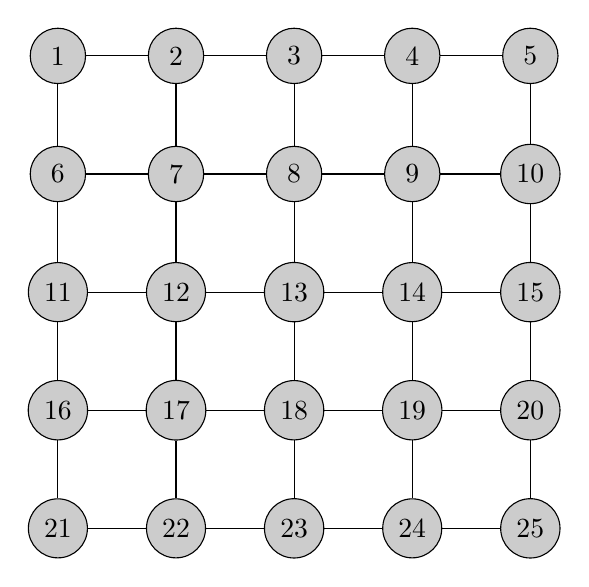
\begin{tikzpicture}[darkstyle/.style={circle,draw,fill=gray!40,minimum size=20}]
  \foreach \x in {0,...,4}
    \foreach \y in {0,...,4} 
       {
       \pgfmathtruncatemacro{\label}{\x - 5 *  \y +21}
       \node [darkstyle]  (\x\y) at (1.5*\x,1.5*\y) {\label};
       } 

  \foreach \x in {0,...,4}
    \foreach \y [count=\yi] in {0,...,3}  
      \draw (\x\y)--(\x\yi) (\y\x)--(\yi\x) ;

\end{tikzpicture}
\end{frame}
%*****************************************************************************
\tikzfeynmanset{
% every vertex={red, dot},
% every particle={blue},
every blob={draw=green!40!black, pattern color=green!40!black},
}
%*****************************************************************************
\begin{frame}{Feynman digrams}
% \begin{tikzpicture}
% \begin{feynman}
% \vertex [blob] (v1);
% \vertex [above left=of v1] (i1) {\(\overline q\)};
% \vertex [below left=of v1] (i2) {\(q\)};
% \vertex [right=of v1] (v2);
% % \vertex [above right=of b] (f1) {\(\nu_{\mu}\)};
% % \vertex [below right=of b] (c);
% % \vertex [above right=of c] (f2) {\(\overline \nu_{e}\)};
% % \vertex [below right=of c] (f3) {\(e^{-}\)};
% \diagram* {
% (i2) -- [fermion] (v1),
% (v1) -- [fermion] (i1),
% % [blob] (v2) -- [boson, edge label'=\(W\)] (v1),
% % (v1) -- [boson, edge label'=\(W\)] (v2),
% % (a) -- [fermion] (b) -- [fermion] (f1),
% % (b) -- [boson, edge label'=\(W^{-}\)] (c),
% % (c) -- [anti fermion] (f2),
% % (c) -- [fermion] (f3),
% };
% \end{feynman}
% \end{tikzpicture}

% \feynmandiagram [horizontal=a to b] {
% a [particle={\(\gamma, Z\)}] -- [boson] b [blob],
% c -- [fermion] b -- [fermion] d,
% };

\feynmandiagram [inline=(b), horizontal=a to b] {
a -- b -- {c [particle=\(c\)], d [particle=\(d\)]}
};
\end{frame}
%*****************************************************************************
%*****************************************************************************
\begin{frame}{INSERTED PAGE NEXT SLIDE}
 
\end{frame}
%*****************************************************************************
%*****************************************************************************
{
\setbeamercolor{background canvas}{bg=}
\includepdf[pages=14]{lucid15_feb11.pdf}
}
%*****************************************************************************
\backupbegin
%*****************************************************************************
\begin{frame}{\large BACKUP}
 
\end{frame}
%*****************************************************************************
\backupend

\end{document}

